%----------------------------------------------------------------------------------------
%	PACKAGES AND OTHER DOCUMENT CONFIGURATIONS
%----------------------------------------------------------------------------------------

\documentclass[a4paper]{scrartcl}
\usepackage[english]{babel}
\usepackage[utf8]{inputenc}
\usepackage{amsmath}
\usepackage{graphicx}
\usepackage{caption}
\usepackage{subcaption}
\usepackage{xargs}                      % Use more than one optional parameter in a new commands
\usepackage[pdftex,dvipsnames]{xcolor}  % Coloured text etc.
\usepackage[colorinlistoftodos,prependcaption,textsize=tiny]{todonotes}
\newcommandx{\unsure}[2][1=]{\todo[linecolor=red,backgroundcolor=red!25,bordercolor=red,#1]{#2}}
\newcommandx{\change}[2][1=]{\todo[linecolor=blue,backgroundcolor=blue!25,bordercolor=blue,#1]{#2}}
\newcommandx{\info}[2][1=]{\todo[linecolor=OliveGreen,backgroundcolor=OliveGreen!25,bordercolor=OliveGreen,#1]{#2}}
\newcommandx{\improvement}[2][1=]{\todo[linecolor=Plum,backgroundcolor=Plum!25,bordercolor=Plum,#1]{#2}}
\newcommandx{\thiswillnotshow}[2][1=]{\todo[disable,#1]{#2}}

\addtokomafont{disposition}{\rmfamily}

\usepackage{footnote}
\makesavenoteenv{figure}

\usepackage[babel,english=british]{csquotes} % cool quotes
\usepackage[backend=biber]{biblatex} % bibliogrpahy
\addbibresource{literature.bib}

\begin{document}

\title{fMRI: BOLD-Contrast and neural activity imaging}
\subtitle{Master Pflichtseminar}
\author{Lucas-Raphael Müller}
% \date{\today}
\maketitle

\begin{abstract}
Your abstract.
\end{abstract}

\tableofcontents

% \newpage

\listoftodos[Notes]

\newpage

\section{Introduction}
\label{sec:intro}

\subsection{Outline}
\subsection{What's the aim?}

\section{Physiology}
Not only is the knowledge of the functional structure of the human brain a major issue for neuroscientists, it's vast complexity is also fascinating for almost everyone.
Major parts of the brain consists of neurons. 
Biophysical aspects are understood on a neuron-wise context, membrane potentials, ion channels and signal propagation are topics to be found in all physiology books which are worth the paper they have been printed on.\cite[577 et. seq.]{guyton}
% Commands to include a figure:
\begin{figure}[hbt]
  \begin{subfigure}[l]{0.35\textwidth}
    \includegraphics[width = \textwidth]{pictures/largeNeuron.png}
    \subcaption{Structure of a large neuron in the brain showing it's important functional parts.\cite[578]{guyton}}
  \end{subfigure}
  \begin{subfigure}[r]{0.6\textwidth}
    \includegraphics[width = \textwidth]{pictures/signalProcessing.png}
    \subcaption{Top row: hypothetical plots of average neuronal activity over time. Bottom row: corresponding functional magnetic resonance imaging (fMRI) responses. Left: hypothetical haemodynamic impulse response function (HIRF) measured as the response to a brief pulse of neuronal activity. Right: the fMRI response when the average neuronal activity alternates (at specific times) between three different states.\cite{Heeger2002}}
    \end{subfigure}
  \caption{Zwei Bilder mit Subfigure nebeneinander.}
\end{figure}
\change{Change Figure 1: Zwei Bilder mit Subfigure....}
Being aware that a physical description is possible on a microscopic scale, it is a task of huge complexity to describe neural activity in total.
Direct measurement of neural activity, i.e. placing eletrodes directly in the brain, requires surgery and most of the time this can only be done in animal experiments. 
Information can be received at the scalp of the brain, however this is a rather rough estimation and not useful for drawing precise activation maps.\cite[6]{buxton}
Modern approaches are positron emission tomography (PET) or funtional magnetic resonance imaging among others.
These methods rely on a implicit measurement, as no electrical field or voltage drop is measured, but other quantities which are followup-like, namely glucose consumption or blood oxygenation level, which are again measured implicitly.
In the former case, tracers with glucose accumulate in regions of high glucose consumption resulting in a local higher active radiation source.
In the latter case, blood oxygenation level changes local inhomogenities of the magnetic field and leads to different \textit{$T_2^*$} relaxation.
The author wants to focus on aspects of the latter one and shortly describe important underlying principles as well as the most basic but necessary physiological knowledge.
With ongoing progress in medical physics research promising measurement method \textit{Magnetoencephalography (MEG)} with great spatial and temporal resolution is mentioned briefly in \ref{sec:outlook}. 

\subsection{Neural Activity}


Notes:
Deoxy is paramagnetic, induces magnetic field inhomogenity \\
Oxy is diamagnetic, no influence \\
Cerebal blood flow. Brain activity -. blood flow -. oxygenated hemoglobin -. $T_2^*$ -. MRI signal\change{Only thoughts}

\subsection{Magnetic Properties}
\label{sub:magneticProperties}
The magnetic properties of hemoglobin and it's related substances were described by Pauling and Coryell in 1936.\cite{pauling}\improvement{Add information to pauling, journal etc.}
Deoxygenated hemoglobin is paramagnetic since the iron atom is ionically bound and four unpaired electrons are present per hemoglobin-group. 
As shown in figure \ref{fig:bindingHb}, oxygenated hemoglobin we see a covalent iron binding structure and no unpaired electrons, therefore oxygenated hemoglobin behaves diamagnetic.\cite{Zborowski}
\begin{figure}[hb]
  \centering
  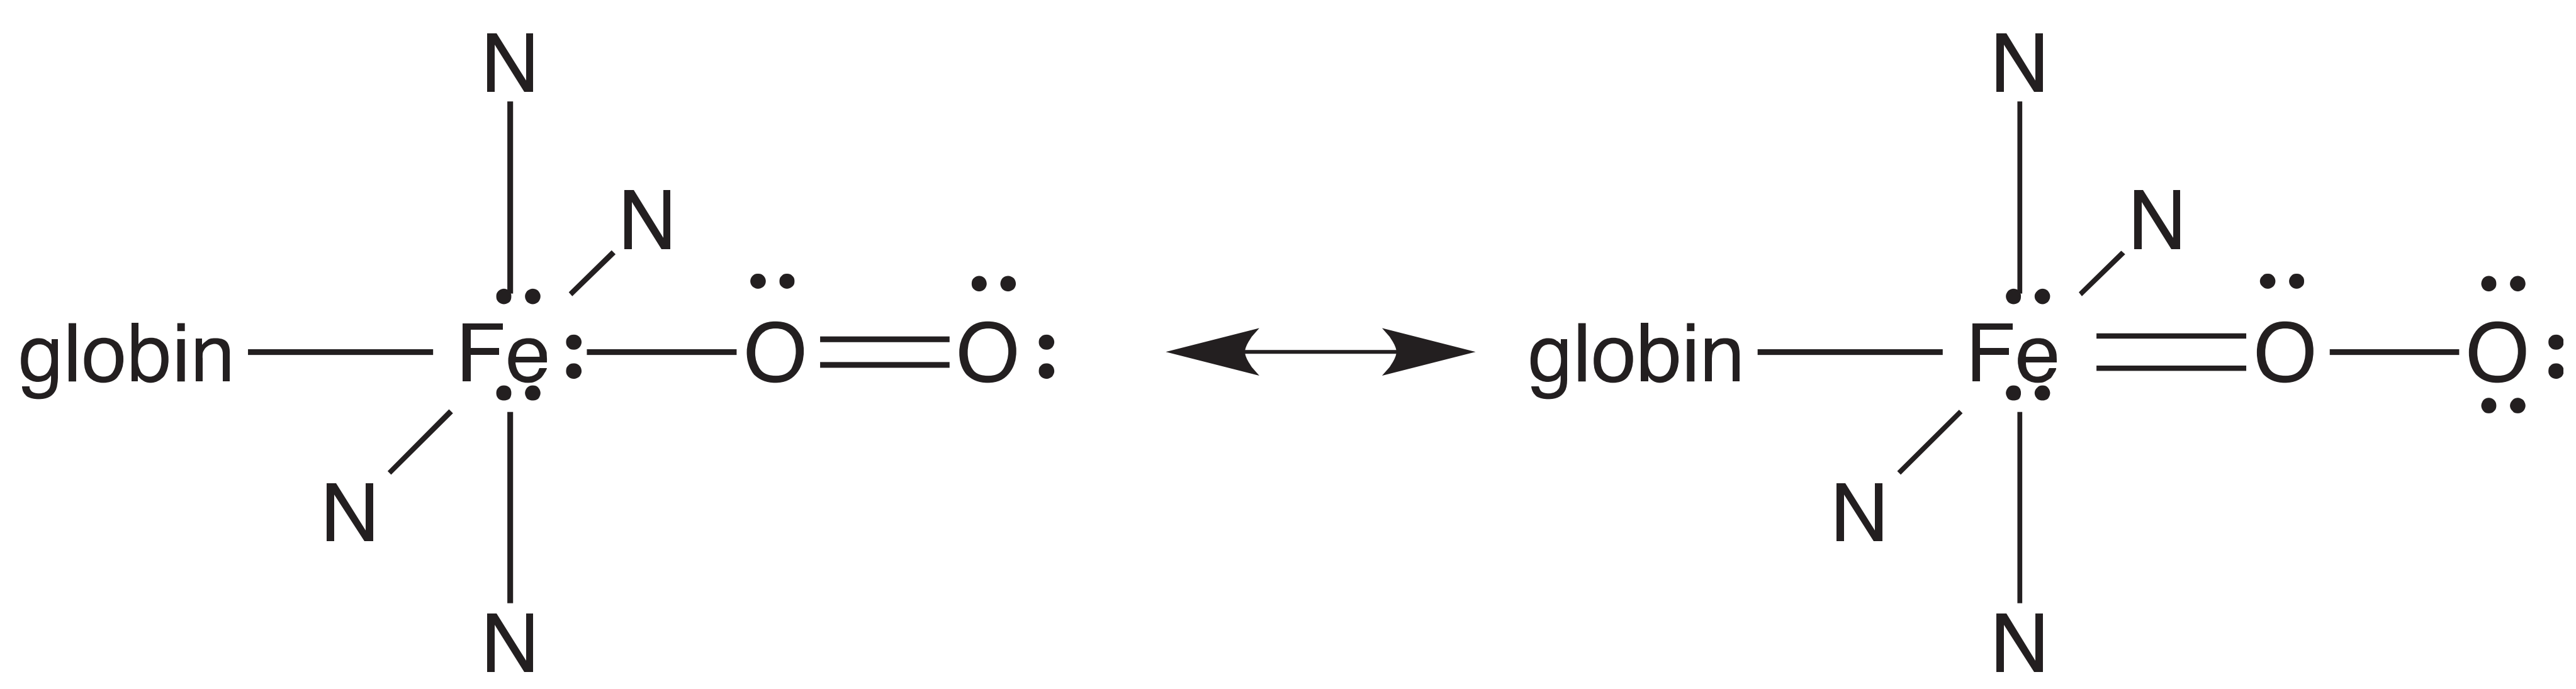
\includegraphics[width = .9\textwidth]{pictures/hemoglobinOxyMagnetic.png}
  \caption{Binding structure of oxyhemoglobin and desoxyhemoglobin.\cite[2]{Bren}}
  \label{fig:bindingHb}
\end{figure}
XXX\improvement{Ask Max which is what.}
This is the very difference which leads to a deviation in the measured signal between deoygenated hemoglobin and oxygenated hemoglobin.
A paramagnet leads to a stronger distortion of the local magnetic field than a diamagnetic behaviour, therefor a signal decrease because of stronger $T_2^*$ decay due to faster dephasing.
measured as image contrast by the MRI machine. As shown in figure \change{Add sequence / relaxation figure or reference it.} 

\section{Hardware}
\label{sec:hardware}

\section{Sequence and Signal}
\label{sec:sequenceSignal}

The usefulness of a neuronal activity map does come with not only spatial but also temporal resolution.
Therefore parameterspace is limited to this constraint.\change{does not sound good}
We also need to limit parameters further, according to section \ref{sub:magneticProperties}. 
We want to \textit{$T_2^*$ - weight} the image and account for local inhomogenities one can eliminate using Spin-Echo sequence.\improvement{wording}

\subsection{Echo Planar Imaging Sequence}
\label{sub:epi}

Incorporating the requirements raised above (introduction section \ref{sec:sequenceSignal}) the author wants to draw the line from SE to EPI sequence.\improvement{Sounds strange.}
\begin{figure}[hbt]
  \centering
  \begin{subfigure}[l]{0.45\textwidth}
    \includegraphics[width = .9\textwidth]{pictures/seSeq.png}
    \subcaption{Spin Echo Sequence with 90 and 180 degree flip.\cite[53]{weishaupt}}
  \end{subfigure}
  \centering
  \begin{subfigure}[r]{0.45\textwidth}
    \includegraphics[width = .9\textwidth]{pictures/episeq.png}
    \subcaption{Echo Planar Imaging Sequence. No 180 degree flip, de and rephasing with rapidly switching frequency gradients. One complete slice per excitation.\cite[59]{weishaupt}}
    \end{subfigure}
  \caption{Spin Echo and Echo Planar Imaging Sequence. Taken from Weishaupt et. al, 'Wie funktioniert MRI?'\cite{weishaupt}}
\end{figure}
Citationstyle\unsure{Unsure citation style.}
Going back to the very basic Spin Echo sequence (by Erwin Hahn \cite{hahn}) one uses a time excessiv 180 degree pulse to refocus magnetic moments and eliminate local inhomogenities.
In this sequence one \textit{line} of constant phase in fourier-space is acquired at a time.
This sequence is time consuming due to the use of the 180 degree pulse and the serial acquisation of \textit{lines} in 2D fourier space, therefore one can not use this sequence for BOLD contrast, since (1) one wants to account for local inhomogenities (free induction decay, $T_2^*$) and (2) the SE is too slow to fullfil the requirement of reasonable temporal resolution.


\section{Software}
\label{sec:software}


\section{Real example (me)}
\label{sec:example}

\section{Outlook}
\label{sec:outlook}

\newpage
\printbibliography

\end{document}

\begin{table}
\centering
\begin{tabular}{l|r}
Item & Quantity \\\hline
Widgets & 42 \\
Gadgets & 13
\end{tabular}
\caption{\label{tab:widgets}An example table.}
\end{table}
